The general second degree equation is expressed as follows,
\begin{align}
    \vec{x^TVx}+2\vec{u^Tx}+f=0\label{eq:solutions/3/4/4/eq:gen}
\end{align}
Comparing \eqref{eq:solutions/3/4/4/eq:given} and \eqref{eq:solutions/3/4/4/eq:gen}, we get
\begin{align}
    \vec{V}=\myvec{ 1 & \sqrt{3} \\ \sqrt{3} & -1 }\label{eq:solutions/3/4/4/eq:V}\\
    \vec{u}=\myvec{0 \\ 0}\label{eq:solutions/3/4/4/eq:u}\\
    f=-2a^2\label{eq:solutions/3/4/4/eq:f}
\end{align}
Now we find
\begin{align}
    \mydet{\vec{V}}=\mydet{1 & \sqrt{3} \\ \sqrt{3} & -1}\\
    \implies\mydet{\vec{V}}=-4\\
    \implies\mydet{\vec{V}}<0
\end{align}

Therefore the given equation \eqref{eq:solutions/3/4/4/eq:given} represents  hyperbola.

Now from affine transformations,
\begin{align}
    \vec{x}=\vec{Py}+\vec{c}
\end{align}

We have to rotate the axes by $\theta=30\degree$, Then using rotation matrix.
\begin{align}
    \vec{P}=\myvec{\cos\theta & -\sin\theta \\ \sin\theta & \cos\theta}
\end{align}
\begin{align}
    \implies\vec{P}=\myvec{\cos30\degree & -\sin30\degree \\ \sin30\degree & \cos30\degree}\\
    \implies\vec{P}=\myvec{\frac{\sqrt{3}}{2} & -\frac{1}{2} \\ \frac{1}{2} & \frac{\sqrt{3}}{2}}\label{eq:solutions/3/4/4/eq:P}
\end{align}

From eigenvalue decomposition,
\begin{align}
    \vec{P^TVP}=\vec{D}\label{eq:solutions/3/4/4/eq:eigval}
\end{align}
\begin{align}
    \implies\vec{D}=\myvec{\frac{\sqrt{3}}{2} & \frac{1}{2} \\ -\frac{1}{2} & \frac{\sqrt{3}}{2}}\myvec{1 & \sqrt{3} \\ \sqrt{3} & -1}\myvec{\frac{\sqrt{3}}{2} & -\frac{1}{2} \\ \frac{1}{2} & \frac{\sqrt{3}}{2}}\\
    \implies\vec{D}=\myvec{2 & 0 \\ 0 & -2}=\myvec{\lambda_1 & 0 \\ 0 & \lambda_2}\label{eq:solutions/3/4/4/eq:D}
\end{align}
\begin{align}
    \vec{P}=\myvec{\vec{p_1} & \vec{p_2}}\\
    \vec{P}^T=\vec{P}^{-1}
\end{align}

The equation \eqref{eq:solutions/3/4/4/eq:gen} becomes as below due to affine transformation
\begin{align}
    \vec{y}^T\vec{Dy}=\vec{u}^T\vec{V}^{-1}\vec{u}-f\label{eq:solutions/3/4/4/eq:trans}
\end{align}
with 
\begin{align}
    \vec{c}=-\vec{V}^{-1}\vec{u}\label{eq:solutions/3/4/4/eq:ctrans}
\end{align}
\begin{figure}[ht!]
    \centering
    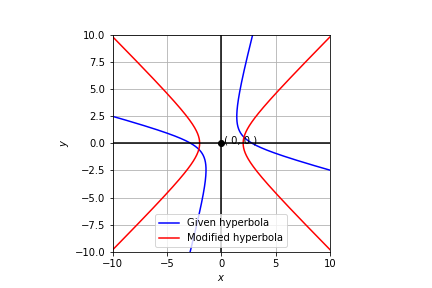
\includegraphics[width=\columnwidth]{./solutions/3/4/4/Figure}
    \caption{For $a=2$, Hyperbola rotated by $30\degree$}
    \label{eq:solutions/3/4/4/fig:figure1}
\end{figure}\\
Substitute \eqref{eq:solutions/3/4/4/eq:V},\eqref{eq:solutions/3/4/4/eq:u},\eqref{eq:solutions/3/4/4/eq:f},\eqref{eq:solutions/3/4/4/eq:D} in \eqref{eq:solutions/3/4/4/eq:trans} and \eqref{eq:solutions/3/4/4/eq:ctrans}, we get
\begin{align}
    \vec{y}^T\myvec{2 & 0 \\ 0 & -2}\vec{y}=2a^2\label{eq:solutions/3/4/4/eq:T}
\end{align}
with centre,
\begin{align}
    \vec{c}=\myvec{0 \\ 0}
\end{align}

Therefore the given equation \eqref{eq:solutions/3/4/4/eq:given} becomes \eqref{eq:solutions/3/4/4/eq:T} when the axes are turned through $30\degree$.

The plot is shown in Fig ~\ref{eq:solutions/3/4/4/fig:figure1} for a=2.
